\documentclass[a4wide, 11pt]{article}
\usepackage{a4, fullpage, hyperref, graphicx}
\usepackage[section]{placeins}
\setlength{\parskip}{0.3cm}
\setlength{\parindent}{0cm}
\graphicspath{ {./images/} }

% This is the preamble section where you can include extra packages etc.

\title{\vspace{-2.0cm}Human Centred Design Techniques Report}

\author{\vspace{-2.0cm}Group 14}

\date{\vspace{-2.0cm}\today}         % inserts today's date

\begin{document}

\maketitle            % generates the title from the data above

% In a few short paragraphs you should discuss and reflect on the Human Centred Design techniques
% that you employed as part of the project. In particular you should discuss your initial research
% into your problem statement (identification of the current state, key design insights and your
% proposed future state) and the HCD Research Methodology employed during the project iterations.
% Additionally, you should diagrammatically evidence the impact of user feedback on your project
% direction during each of the 3 implementation weeks.

\section{HCD Techniques}

\subsection{Initial Research into Problem Statement}

We decided to address the problem of a lack of quality programming education for Key Stage 3 students. After initial research we found that many schools are struggling to keep up with new the UK computing curriculum (figure 1), where students are now taught Computing from 11-14 as a compulsory course, as there is a lack of skilled programming teachers.

Many existing platforms either do not provide facilities for teachers to see student solutions or provide feedback, or don't give students any direction when attempting to teach challenging concepts.

We envisaged an engaging web application to help students learn difficult progamming concepts that are not taught by other platforms, without discouraging them with unintuitive syntax. This platform would allow teachers to set exercises for their classes to complete and track their students' progress through the app.

\subsection{HCD Research Methodology}

We started the project by creating: personas for our target audience (Persona section), a stakeholder map showing which groups of people our app will have an effect on (figure 2) and a mood-o-gram for a teacher's typical programming lesson without our app (figure 3).

Each week we employed an HCD methodology, roughly adhering to the following cycle:

\begin{itemize}
  \item Initially, we collate the previous week's feedback. We use it to determine what existing features have been most useful to the users and what new features would give them the most benefit in the coming week.
  \item After determining the key features, we develop a mocked up representation of the features.
  \item Our primary user tester is a teacher, Lucy Glanfield. We present our mocked up features each Tuesday and let her play with them. We note her verbal feedback and observe her interactions to gain valuable information about the current state of the feature. This feedback helps us decide which features are useful from the teacher's perspective. Lucy has also been able to demo the application with some members of her Key Stage 3 classes so that we can also get feedback on the student's user journey.
  \item We aim to implement/improve the most pressing desired features by Thursday morning. This micro-iteration allows us to receive more user feedback and to improve the functionality from the user's perspective.
  \item Thursday and Friday are spent refining new features in preparation for the following week.
\end{itemize}

\section{Appendix}

\subsection{Personas}
\begin{itemize}
  \item Nancy, 34, Chemistry teacher. Nancy has recently been asked to teach programming
  to Key Stage 3 students due to the new curriculum and a shortage of skilled
  Computer Science teachers. She has been given access to the IT suite each week
  and is looking for an intuitive digital tool to help her get the key programming
  concepts across to her students.

  \item Mark, 12, student. Mark is not particularly interested in technology (he enjoys
  Biology and wishes to study Medicine at university), however as part of the English
  curriculum he is required to attend a class teaching many of the core
  Computer Science concepts. Mark wants an engaging learning platform that
  does not require any prior knowledge of programming while still teaching him
  everything he needs to know.
\end{itemize}

\subsection{Figures}

\begin{figure}[h]
  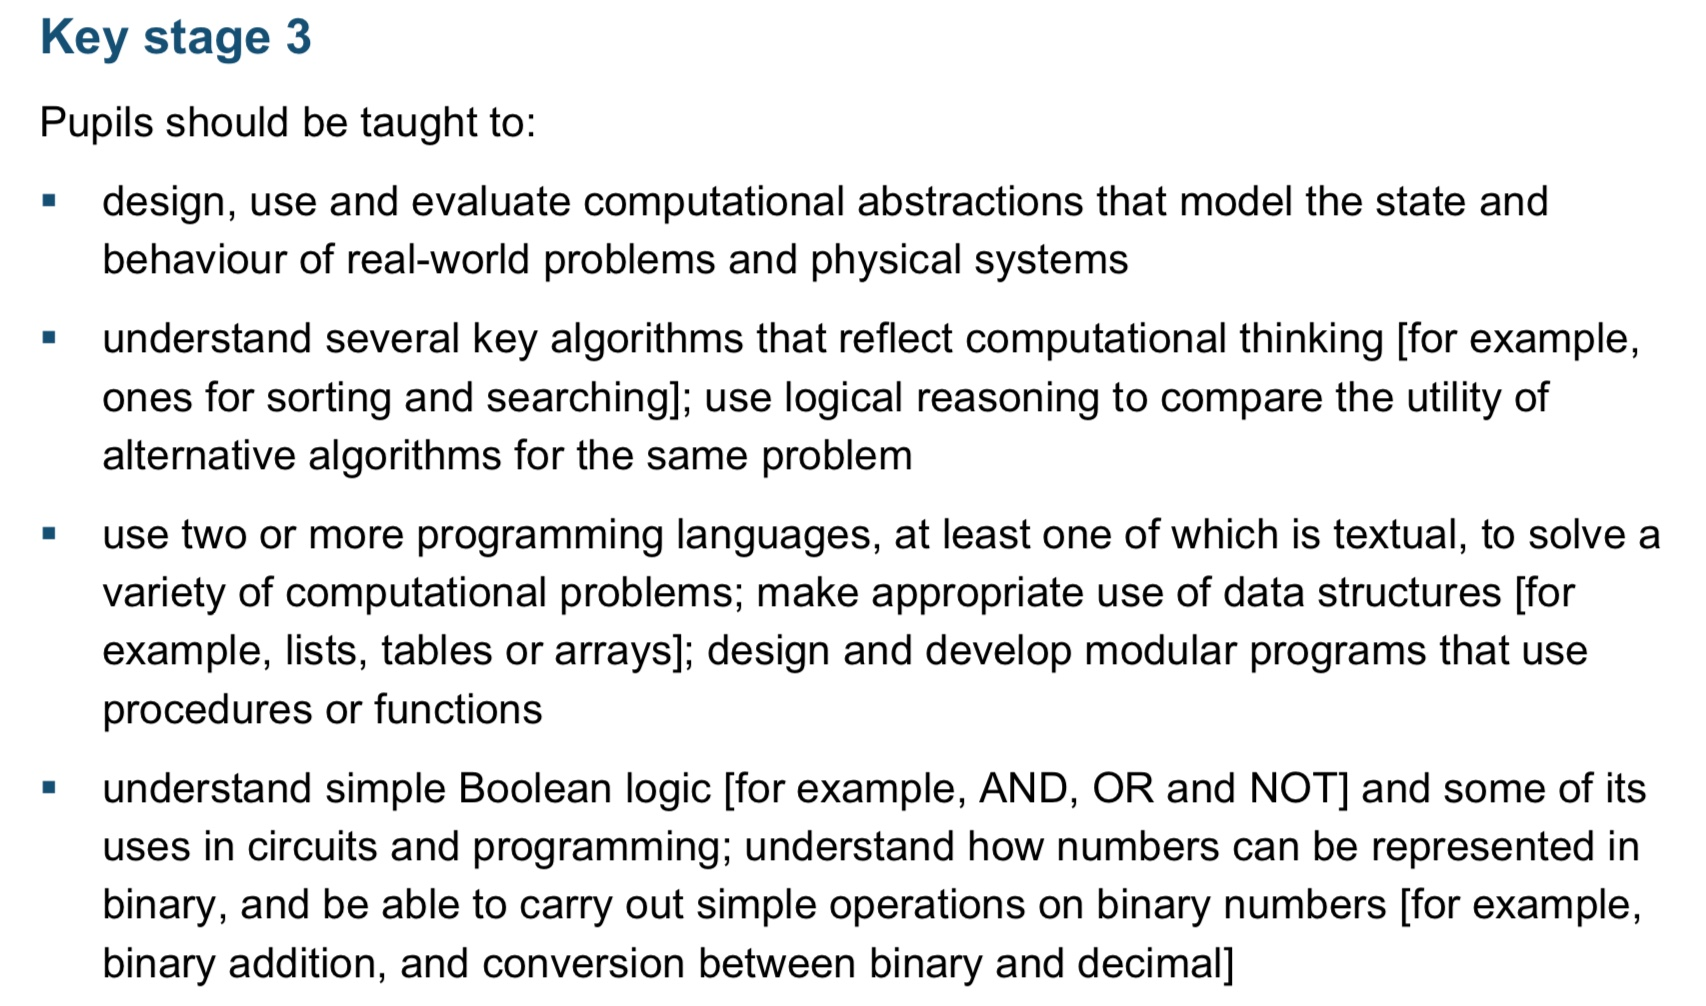
\includegraphics[scale=0.25]{curriculum_extract.jpeg}
  \centering
  \caption{An extract from Comuting curriculum}
\end{figure}

\begin{figure}[h]
  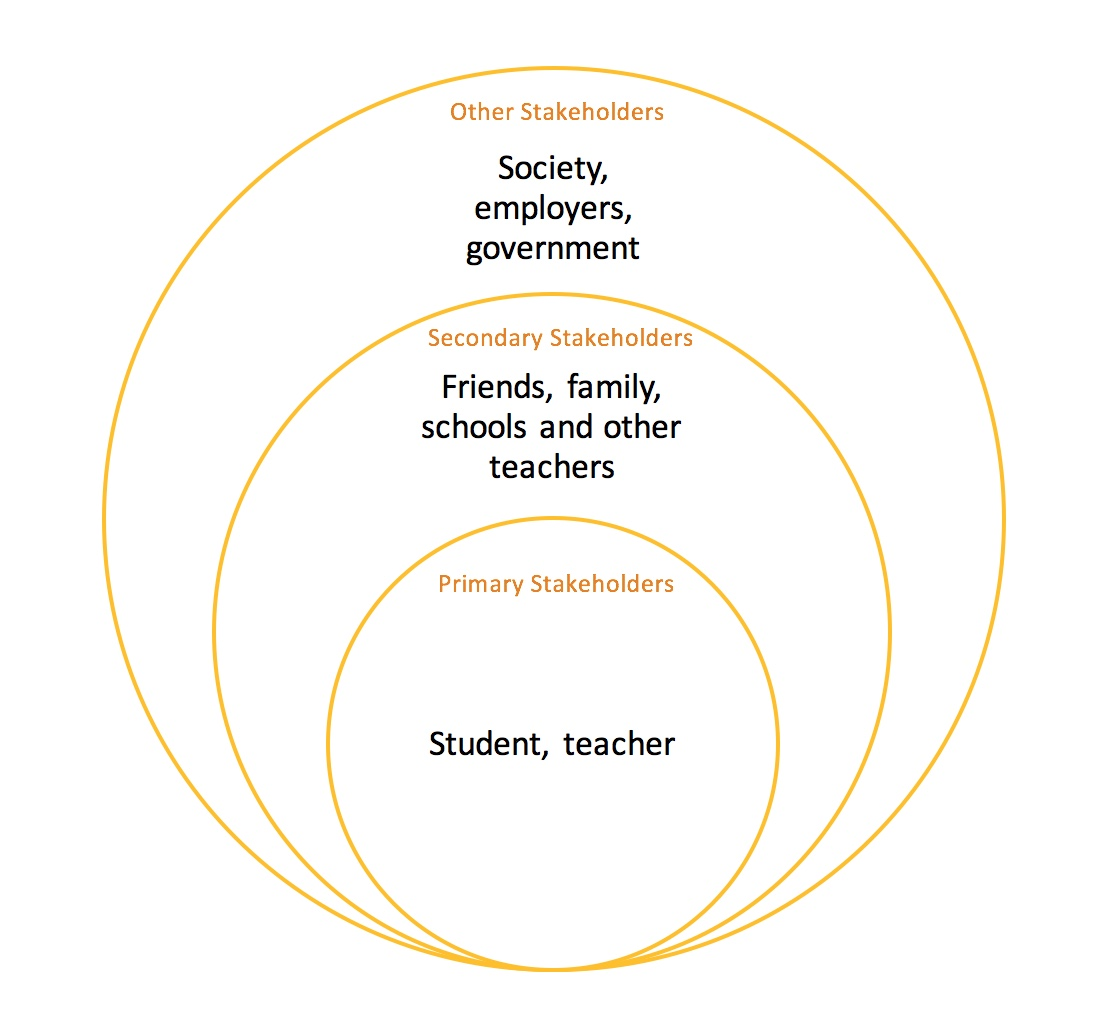
\includegraphics[scale=0.25]{stakeholders.jpeg}
  \centering
  \caption{A stakeholder diagram}
\end{figure}

\begin{figure}[h]
  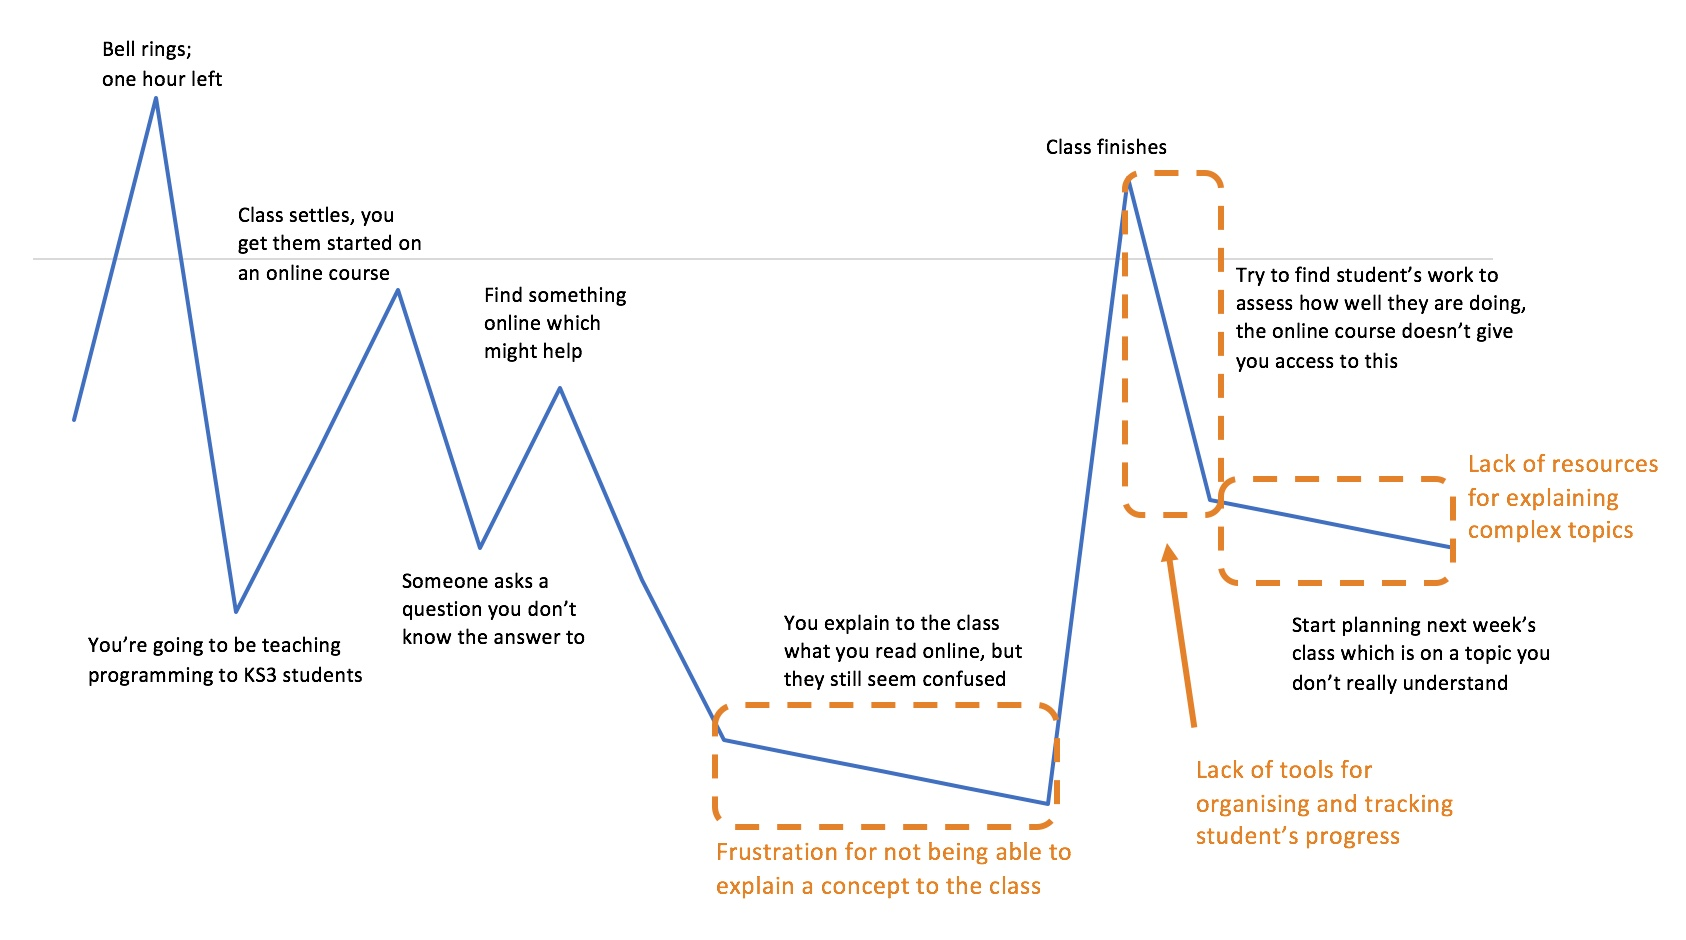
\includegraphics[scale=0.3]{mood-o-gram.jpeg}
  \centering
  \caption{A mood-o-gram for a teacher's typical programming class}
\end{figure}

\begin{figure}[t]
  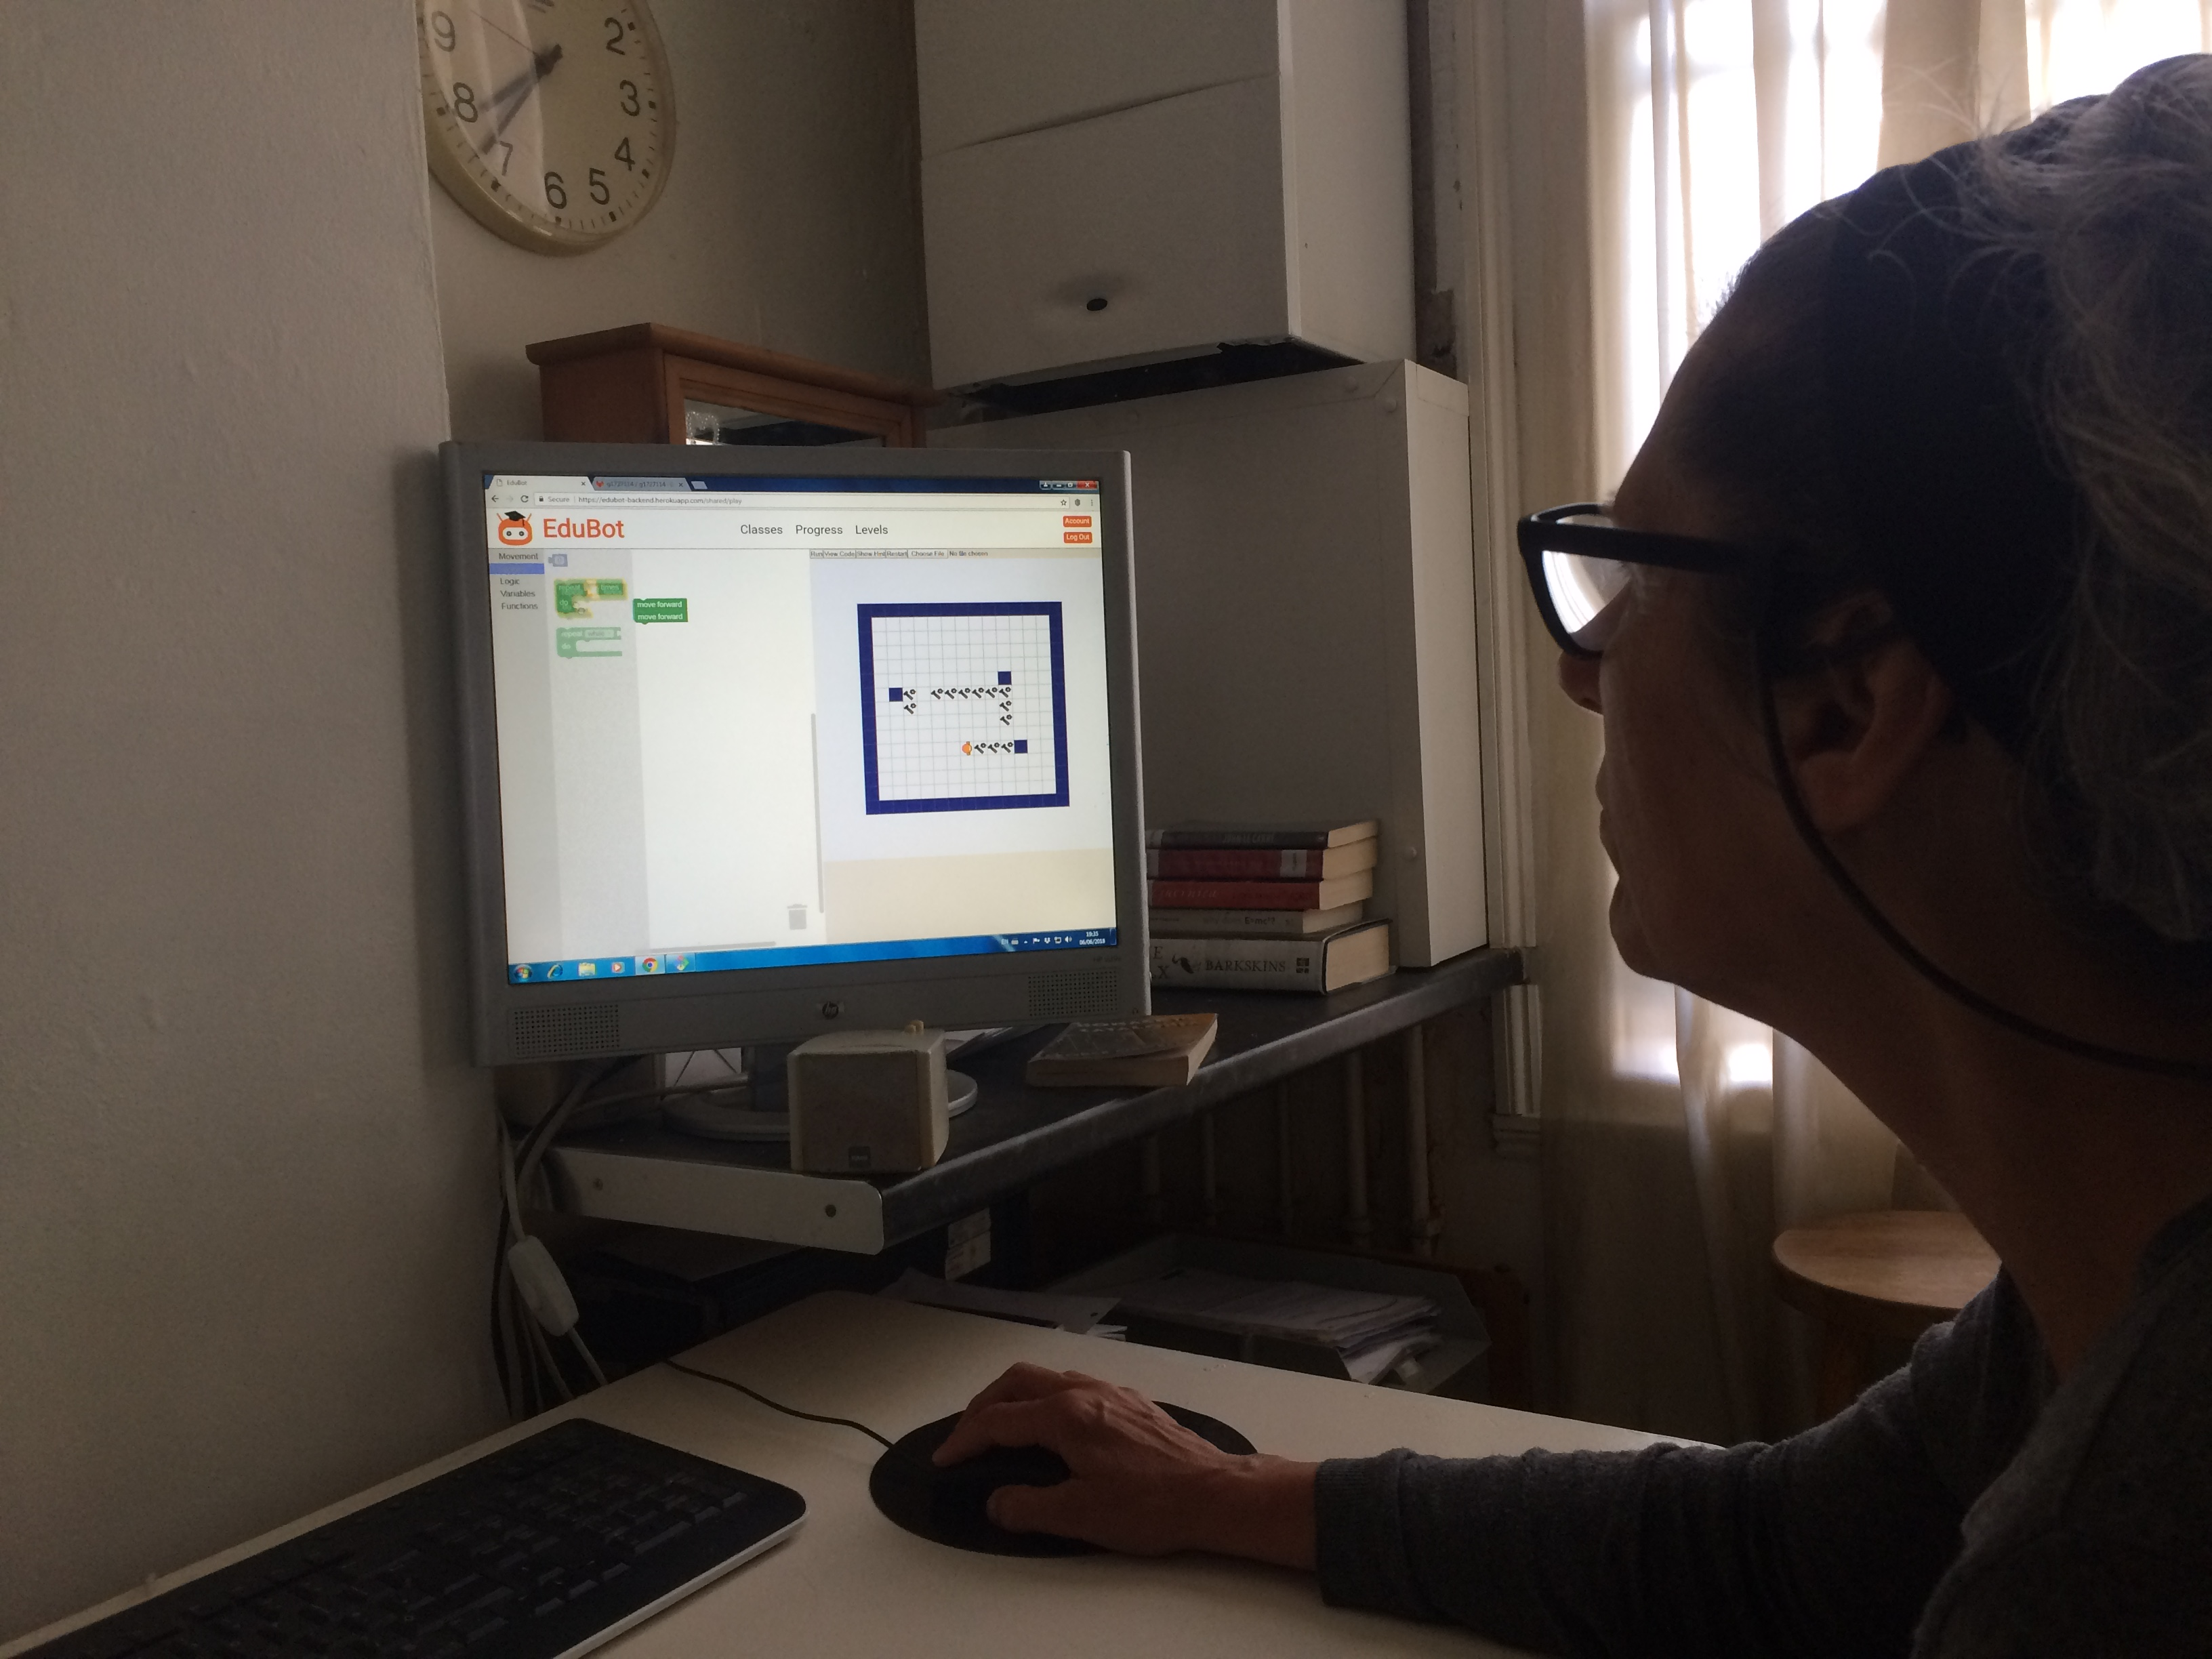
\includegraphics[scale=0.1]{user_feedback_session.JPG}
  \centering
  \caption{Getting feedback from a potential user}
\end{figure}

\FloatBarrier
\subsection{Diagrammatic Evidence of User Feedback}

\begin{figure}[h]
  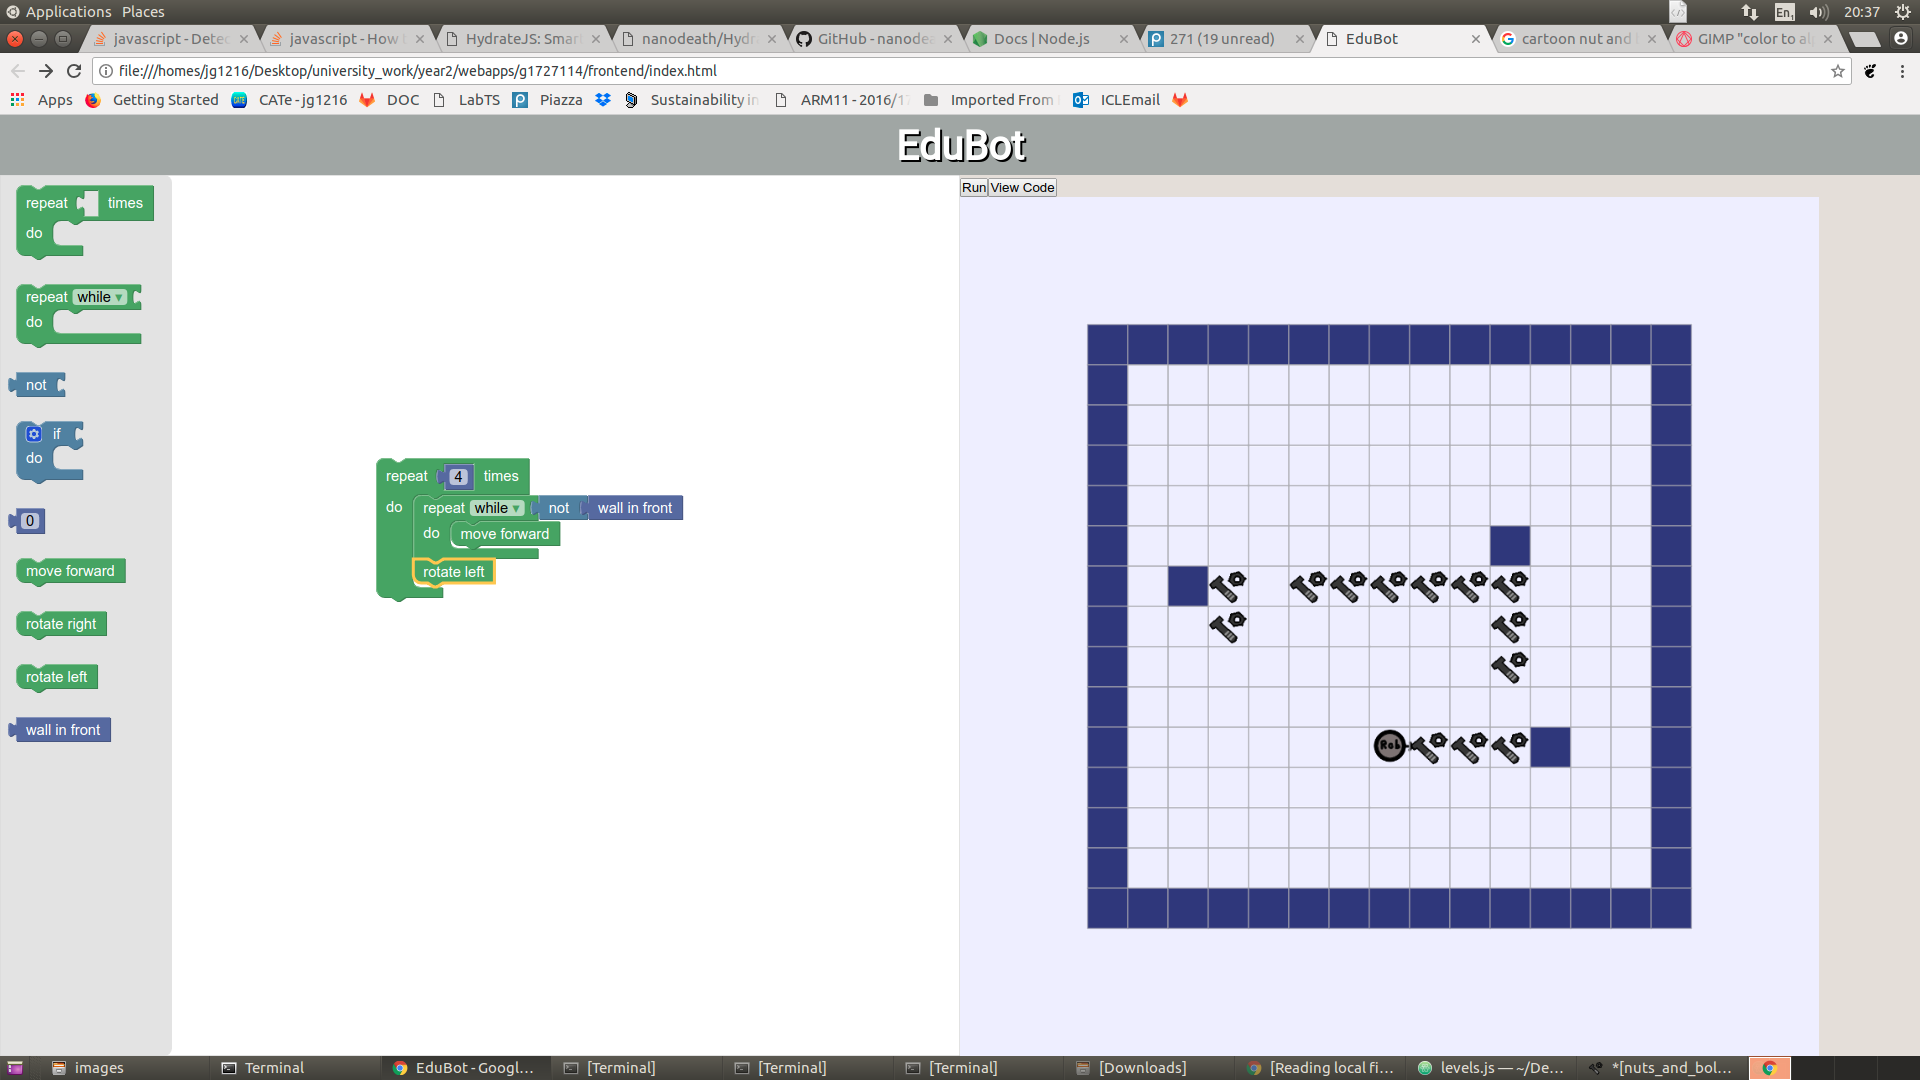
\includegraphics[scale=0.18]{prototype2.png}
  \centering
  \caption{First iteration}
\end{figure}

\begin{figure}[h]
  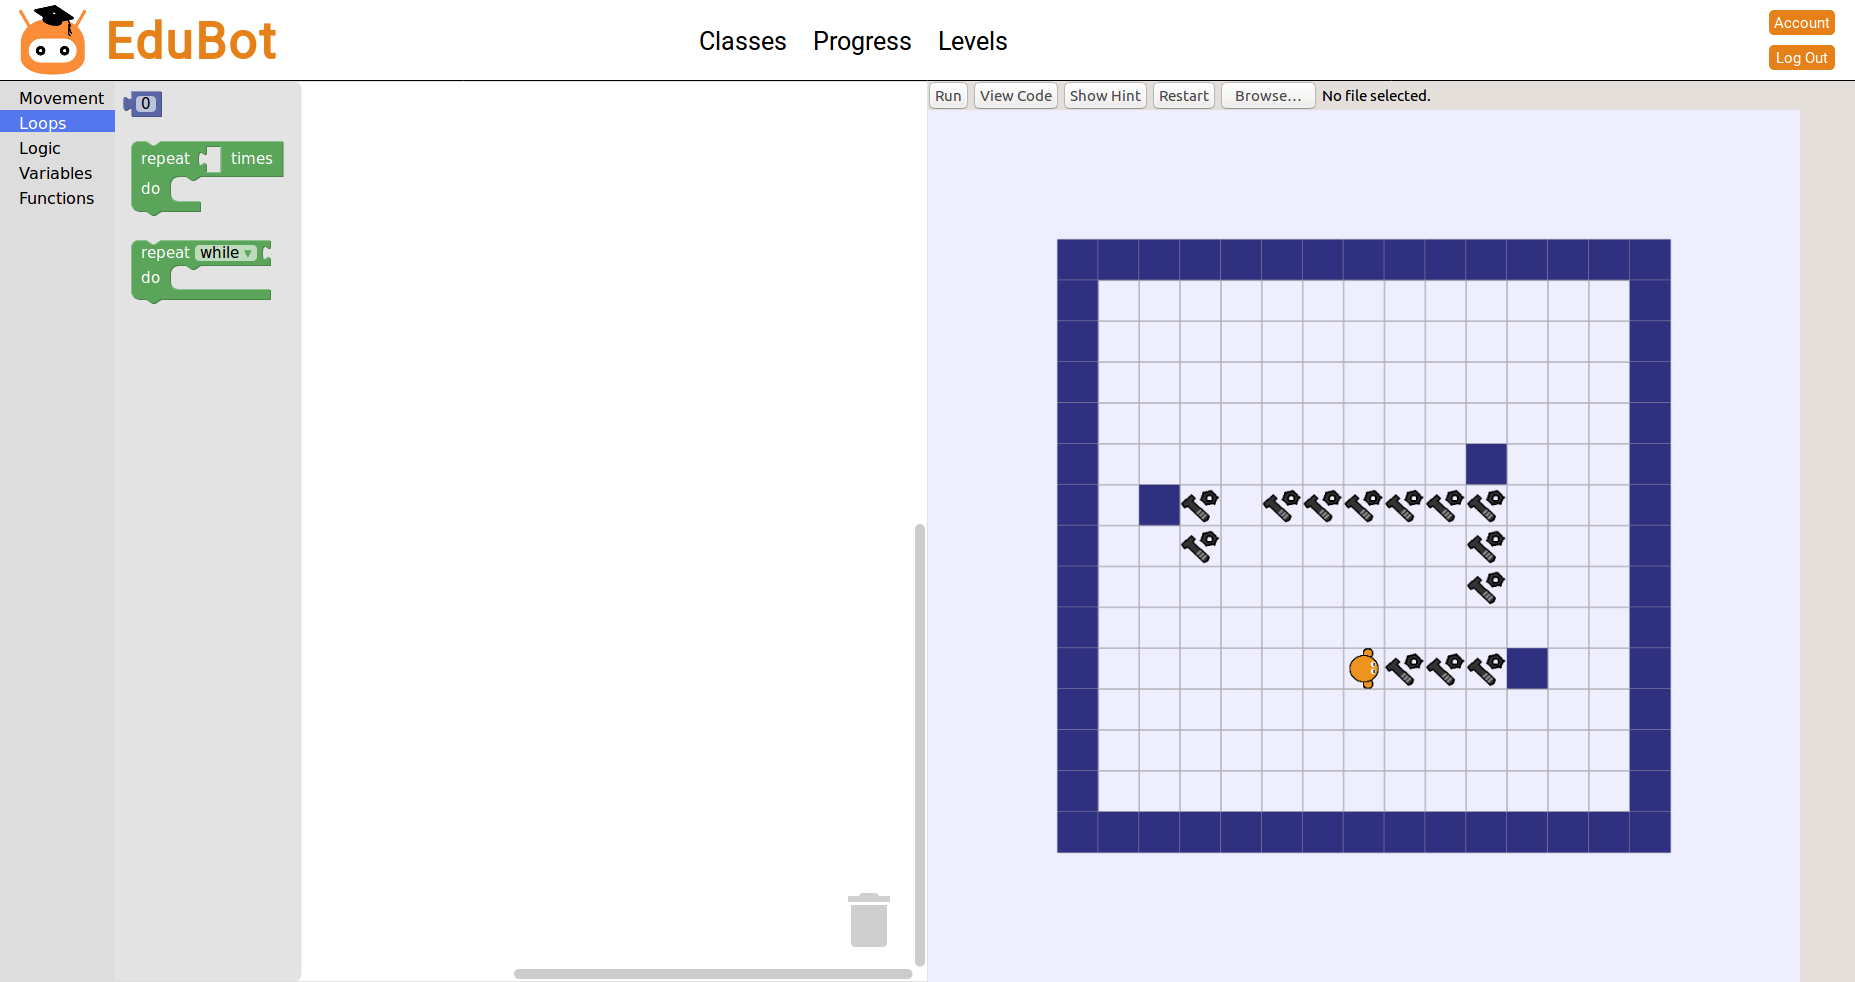
\includegraphics[scale=0.18]{play.png}
  \centering
  \caption{Second iteration}
\end{figure}

\end{document}
